\documentclass[twoside,12pt]{article}

\usepackage{lmodern}
\usepackage[T1]{fontenc}
\usepackage[spanish,activeacute,es-tabla]{babel}
\usepackage{mathtools}
\usepackage{graphicx}
\usepackage[inner=3.0cm,top=2.5cm,outer=2.0cm,bottom=2.5cm]{geometry}  
\usepackage{fancyhdr}
\usepackage{hyperref}
\usepackage{multicol}
\usepackage{glossaries}

\pagenumbering{gobble}
%\renewcommand{\baselinestretch}{1.5}
\usepackage{setspace}
\onehalfspacing

\setlength{\footskip}{42pt}

\title{\begin{center} 

\includegraphics[width=0.8\textwidth]{images/upc-logo.png} 
\end{center} 
\vspace{0.5cm} 
Proyecto Final de Carrera\\
INGENIER\'IA INDUSTRIAL \\
\vspace{0.5cm} 
\Huge{
RosPiBot}
\vspace{0.5cm} \\
 Memoria}

\author{}
\date{} % void to avoid put current date
\pagestyle{fancy}

\fancyhead[LO,RE]{\title{RosPiBot}}
\fancyhead[LE,RO]{\thepage}
\fancyfoot[LE,RO]{
\includegraphics[scale=0.5]{images/etseib-logo.png}}
\fancyfoot[C]{}
%\headrulewidth 0.4pt
%\footrulewidth 0 pt

%\makeglossaries
%\newacronym{IIC}{I$^{2}$C}{Inter-Integrated Circuit}
%\newacronym{SPI}{SPI}{Serial Protocol Interface}
%\newglossaryentry{electrolyte}{name=electrolyte, description={solution able to conduct electric current}}

\begin{document}
%\pagestyle{empty} 

\maketitle
\begin{center}
\large{$\begin{array}{ll}
\mbox{Autor:} & \mbox{Joan Guasch Iglesias} \\
\mbox{Director:} & \mbox{Manel Velasco Garcia} \\
\mbox{Convocatoria:} & \mbox{Fecha a presentar}
\end{array}$}\\ 
\vspace{2cm} 
\Large{Escuela T'ecnica Superior de Ingenier'ia Industrial de Barcelona}\\ 
\vspace{1cm}

\includegraphics[scale=1]{images/etseib-logo.png}
\end{center}
\thispagestyle{empty}
\newpage

\thispagestyle{empty}
\paragraph*{}
\newpage

%\thispagestyle{empty}
%\pagenumber{1}
\pagenumbering{arabic}
\fancyhead[LE,RO]{1} 

\normalsize
\begin{abstract}
Este proyecto consiste en el aprovechamiento de la plataforma rob'otica comercial WifiBot que corre el riesgo de quedarse obsoleta y rescatarla de su destino. Para ello se hace uso de una Raspberry Pi, un ordenador de placa reducida que ha revolucionado el mundo de la automatizaci'on desde el d'ia de su aparici'on en el 2012, como unidad de procesamiento de la nueva plataforma y que est'a basada en Linux. En el apartado de software, adem'as de incorporar herramientas que faciliten el trabajo a futuros usuarios se ha configurado para poder trabajar con ROS, una infrastructura digital para el desarrollo de software de robots creada por Willow Garage y extensamente utilizada en este sector.\\

A lo largo de este documento se exponen el estado inicial del robot, los nuevos requerimientos a cumplir, las modificaciones efectuadas incluyendo las complicaciones encontradas a lo largo del proyecto y el resultado final obtenido. Haciendo especial hincapi'e en el desarrollo de soluciones para cumplir los objetivos del proyecto, tales como el dise'no de circuitos electr'onicos, la integraci'on de los nuevos componentes o la creaci'on de una mejor interf'icie para el usuario. \\

\end{abstract}

%\thispagestyle{empty}
\newpage

\paragraph*{}
\thispagestyle{empty}
\newpage

\fancyhead[LE,RO]{3}
\tableofcontents
\setcounter{page}{1}
\addtocontents{toc}{~\hfill\textbf{P'agina}\par}
\addcontentsline{toc}{section}{Resumen}
%\setcounter{page}{1}
\addcontentsline{toc}{section}{Glosario}
%\setcounter{page}{4}
\fancyhead[LE,RO]{4}
%\setcounter{page}{3}
%\addcontentsline{toc}{section}{'Indice}
\newpage

%\pagenumbering{arabic}
\setcounter{page}{5}
\fancyhead[LE,RO]{\thepage}

\section*{Glosario}
\begin{description}
\item[UART] Universal Asynchronous Receiver-Transmitter
\item[SPI] Serial Protocol Interface
\item[I${2}$C] Inter-Integrated Circuit
\item[ADC] Analog to Digital Converter
\item[SoC] System on a Chip
\item[CPU] Central Processing Unit
\item[GPU] Graphics Processing Unit
\item[RAM] Random Access Memory
\item[RCA] Random Access Memory
\item[HDMI] Random Access Memory
\item[DSI] Random Access Memory
\item[CSI] Random Access Memory
\item[GPIO] Random Access Memory
\item[SD] Random Access Memory
\end{description}

%\printglossaries


\newpage

\section{Introducci'on}

\subsection{Estado del arte}

\subsection{Alcance}


\subsection{Objetivos}

\newpage

\section{Descripci'on }

\subsection{WifiBot}
\textbf{Wifibot} es una plataforma rob'otica, desarrollada por la empresa francesa \textbf{Nexter Robotics}, dise'nada para poder navegar en m'ultiples escenarios gracias a su dise'no. Su sistema de tracci'on a las cuatro ruedas, dise'no reducido y bajo peso, le otorga una gran flexibilidad.

\subsubsection{Caracter'isticas}
Este proyecto parte del modelo \textbf{WifiBot 4G}, producido durante el periodo 2002--2006 y que a grandes rasgos incluye::

\begin{figure}[ht]
\centering
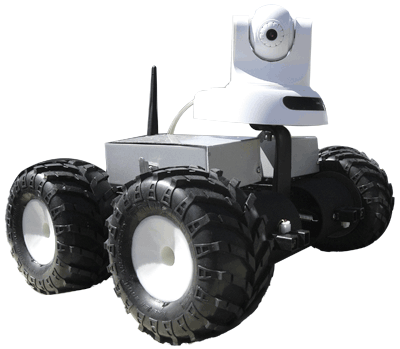
\includegraphics[scale=0.5]{images/Visuel_Wifibot_2.png} 
\caption{Wifi Bot 4G}
\label{fig:Wifi Bot 4G}
\end{figure}

\paragraph*{}

\begin{multicols}{2}
\begin{itemize}
\item CPU:
	\begin{itemize}
	\item Procesador AMD Au1500
	\item 400MHz
	\item Mem'oria RAM de 64MB
	\item Mem'oria Flash de 32MB
	\end{itemize}
\item Interf'icies:
	\begin{itemize}
	\item 4x Ethernet 10/100
	\item 1x USB
	\item 1x I$^{2}$C %\gls{IIC}
	\item 1x RS232
	\end{itemize}
\item WIFI:
	\begin{itemize}
	\item WiFi con est'andar 802.11a/b/g
	\item Modos Access Point, Bridge, Client y Router
	\item 1x Antena de 5dBi
	\end{itemize}
\item Sensores:
	\begin{itemize}
	\item 1x C'amara IP
	\item 2x Sensores IR de dist'ancia (ADC)
	\item 2x Codificadores 'optico de cuadratura 
	\item 2x DSPIC30F2010
	\item 1x Nivel de bater'ia (ADC)
	\end{itemize}
\item Motores:
	\begin{itemize}
	\item 4x Motores de 7.2V
	\item Reductora $i=50:1$
	\item Par nominal 8.87Kg/cm
	\item Velocidad nominal 120Rpm
	\end{itemize}
\item Dimensiones:
	\begin{itemize}
	\item Longitud 28cm
	\item Anchura 30cm
	\item Altura 20cm
	\item Peso 4.5Kg
	\end{itemize}
\item Bater'ias:
	\begin{itemize}
	\item 9.6V NiMh (8 celdas)
	\item Capacidad 9500mAh
	\item Autonom'ia de 2 horas
	\end{itemize}
\end{itemize}
\end{multicols}

\subsubsection{Estructura}

La estructura de la base est'a formada por dos secciones sim'etricas que llamaremos hemisferios izquierdo y derecho. Estas dos partes est'an unidas por una barra roscada que atraviesa transversalmente todo el robot, ofreciendo un eje de rotaci'on entre los dos elementos, cualidad que le otorga una mayor adaptaci'on a superf'icies irregulares.
%include image SolidWorks
%como vemos en figura \ref{fig:Wifi Bot 4G}

\subsubsection{Grupo Motriz}
Los motores que componen el WifiBot son concretamente el modelo \textbf{HN-GH7.2-2414T-50:1} del fabricante \textbf{Hsiang Neng}. Este modelo est'a compuesto por un motor de continua de voltaje nominal de 7.2V y una reductora con relaci'on 50:1. Tal y como se describe en la figura ~\ref{fig:Dimensiones del Motor}, dispone de un eje de 6mm de di'ametro, una longitud de 81.1mm y un di'ametro exterior de 37mm. 

\begin{figure}[ht]
\centering
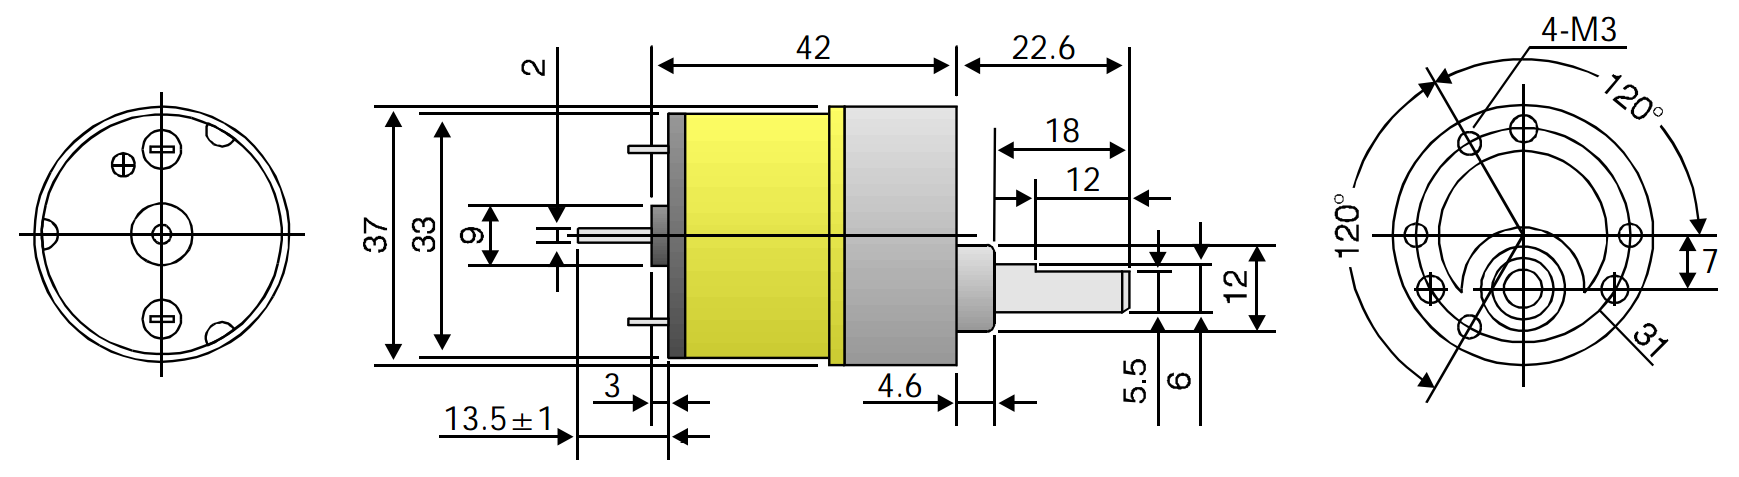
\includegraphics[scale=0.35]{images/motor_dimensions.png} 
\caption{Dimensiones [mm] motor HN-GH7.2-2414T-50:1}
\label{fig:Dimensiones del Motor}
\end{figure}

En mediciones efectuadas, se determin'o que la alimentaci'on de los motores llegaba hasta los 8.2V con un consumo inferior a los 1.8A por motor (con carga), bas'andonos en la figura ~\ref{fig:Gr'afica del Motor}, podremos asegurar que el motor se encontraba ofreciendo un par de 4.7 Kg-cm. 

\begin{figure}[ht]
\centering
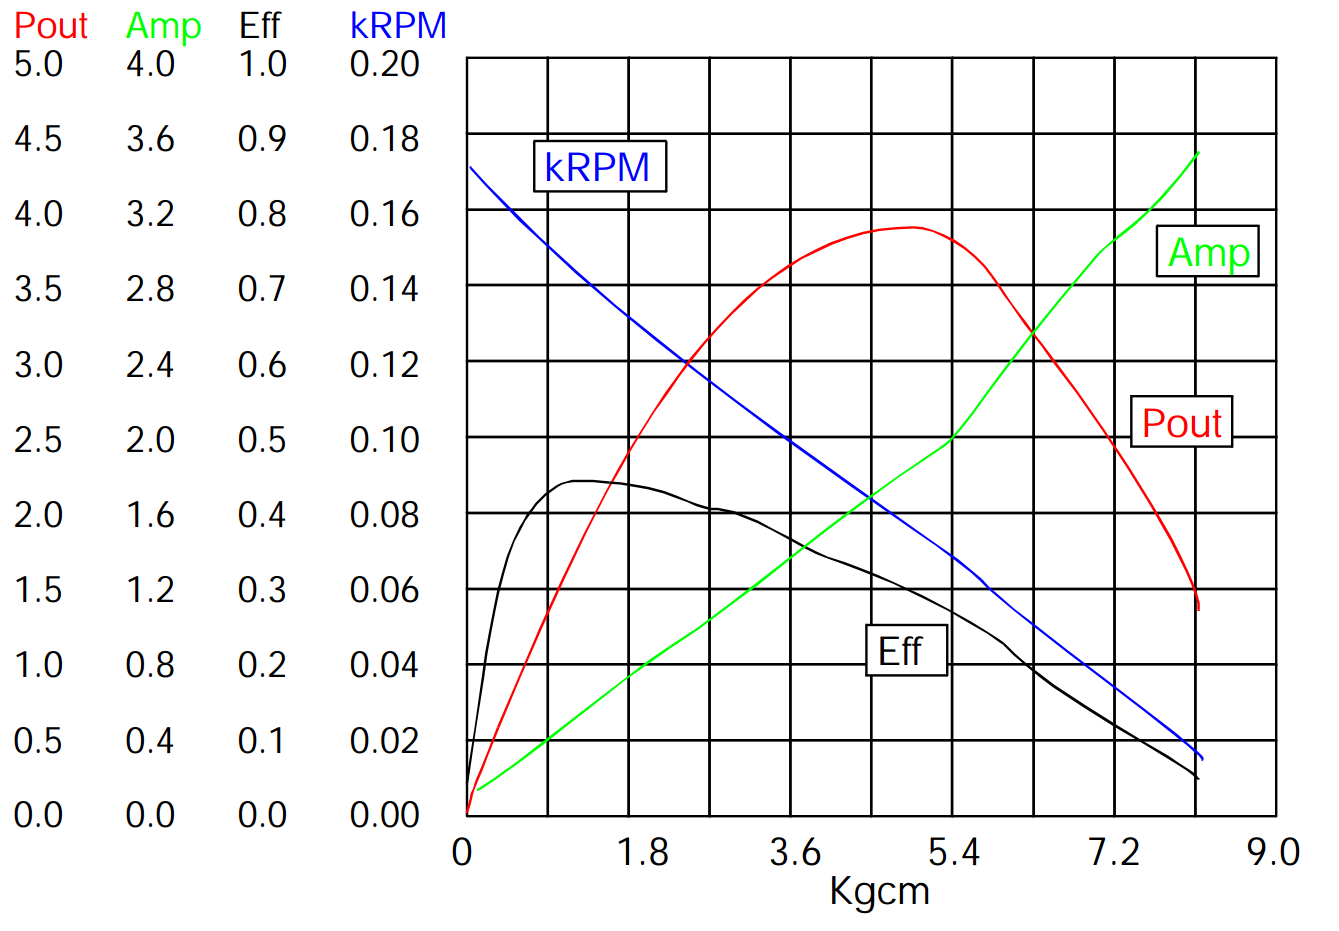
\includegraphics[scale=0.35]{images/motor_graph.png} 
\caption{Gr'afica de curvas espec'ificas del motor HN-GH7.2-2414T-50:1}
\label{fig:Gr'afica del Motor}
\end{figure}

\subsubsection{Codificador 'optico de cuadratura}
Este tipo de sensor permite conocer tanto la velocidad como la posici'on de un eje. Tal y como se describe en la figura ~\ref{fig:Esquema QEI} , su funcionamiento se basa en un disco ranurado que gira solidario al que se dispone un par de fototransistores. Estos transistores emiten una se'nal compuesta por dos canales, com'unmente llamados A y B, de onda cuadrada. Estos dos canales est'an desfasados un cuarto de fase, creando una secuencia que depende del sentido de giro. 

\begin{figure}[ht]
\centering
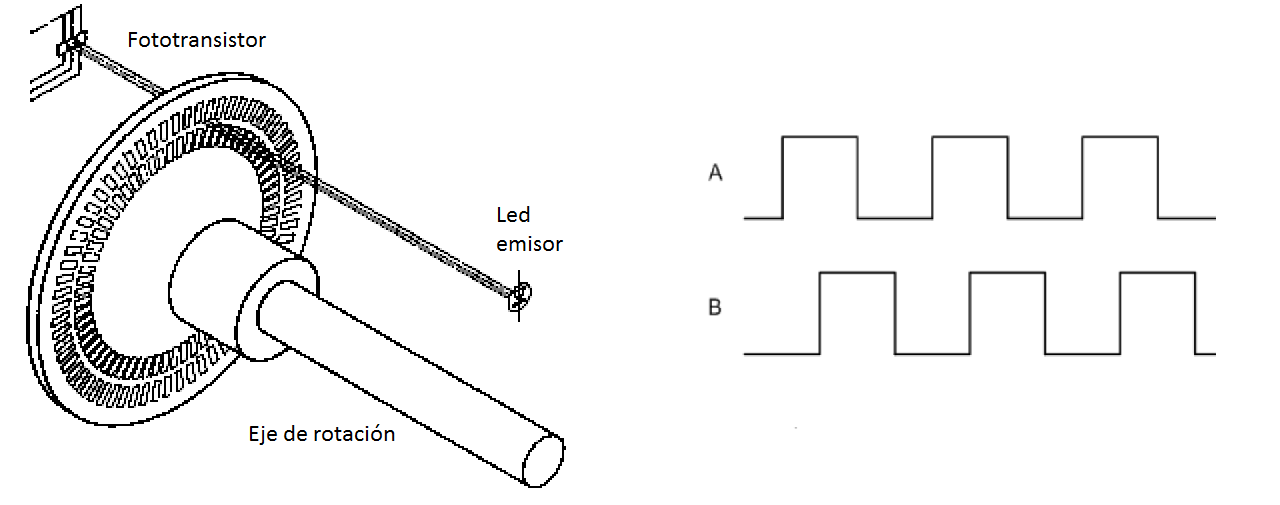
\includegraphics[scale=0.45]{images/encoderQEI.png} 
\caption{Esquema de funcionamiento de un encoder de cuadratura}
\label{fig:Esquema QEI}
\end{figure}

De los 4 motores que conforman la plataforma, los dos delanteros disponen de un codificador 'optico, concretamente el modelo \textbf{E4P-120-079-HT} del fabricante \textbf{US DIGITAL}. Este modelo ofrece unos 120 ciclos por revoluci'on (o 480 interrupciones), est'a pensado para ejes de 2mm de di'ametro y no dispone de canal de 'indice (permite corregir errores). Tras un ensayo del motor sin carga, cuyos datos se encuentran en la tabla ~\ref{tab:Encoder periods}, se determin'o que se llegaba a un m'aximo de 80.000 pulsos por segundo.\\

\begin{table}[ht]
\begin{center}
\begin{tabular}{|c|c|c|}
	\hline
	\textbf{Voltaje [V]} & \textbf{Consumo [A]} & \textbf{Per'iodo de Cuadratura [us]} \\ \hline
	0.5 & 0.07 & 2200 \\ \hline
	1.0 & 0.08 & 1000 \\ \hline
	1.5 & 0.09 & 320 \\ \hline
	2.0 & 0.10 & 220 \\ \hline
	2.5 & 0.11 & 170 \\	\hline
	3.0 & 0.11 & 140 \\ \hline
	3.5 & 0.12 & 120 \\ \hline
	4.0 & 0.12 & 100 \\ \hline  
	4.5 & 0.13 & 90 \\ \hline  
	5.0 & 0.13 & 80 \\ \hline
	5.5 & 0.14 & 70 \\ \hline
	6.0 & 0.15 & 65 \\ \hline
	6.5 & 0.15 & 60 \\ \hline
	7.0 & 0.15 & 55 \\ \hline
	7.5 & 0.16 & 50 \\ \hline

\end{tabular}
\end{center}

\caption{Ensayo de consumo y se'nal de codificador del motor sin carga }
\label{tab:Encoder periods}
\end{table}

\subsubsection{Estado Inicial}  
La plataforma de la que se dispon'ia en un principio carec'ia de cierta cualidades. La m'as destacable era la inestabilidad de la red WiFi, dicha conexi'on sufr'ia constantes ca'idas con lo que dificultaba enormemente su teleopraci'on. Su otro tal'on de Aquiles era su escasa documentaci'on disponible, al ser un producto que su fabricante da por descontinuado y al no disponer de una comunidad que lo mantenga, dicha base rob'otica provocaba quebraderos de cabeza para usuarios noveles. Finalmente, las bater'ias al haber completado su vida 'util, dispon'ian de una carga efectiva muy inferior a la inicial. En cambio, tanto la estructura, ruedas, motores y sensores se encontraban en mejores condiciones\\
\newpage

\subsection{Raspberry Pi}
Raspberry Pi es un ordenador del tama'no de una tarjeta de cr'edito desarrolado en Reino Unido por la \textbf{Raspberry Pi Foundation} con el objetivo de fomentar las bases de la computaci'on en escuelas. El desarrollo de este diminuto ordenador empez'o en el 2006 hasta alcanzar su madurez y comercializaci'on en Febrero del 2012. 

\begin{figure}[ht]
\centering
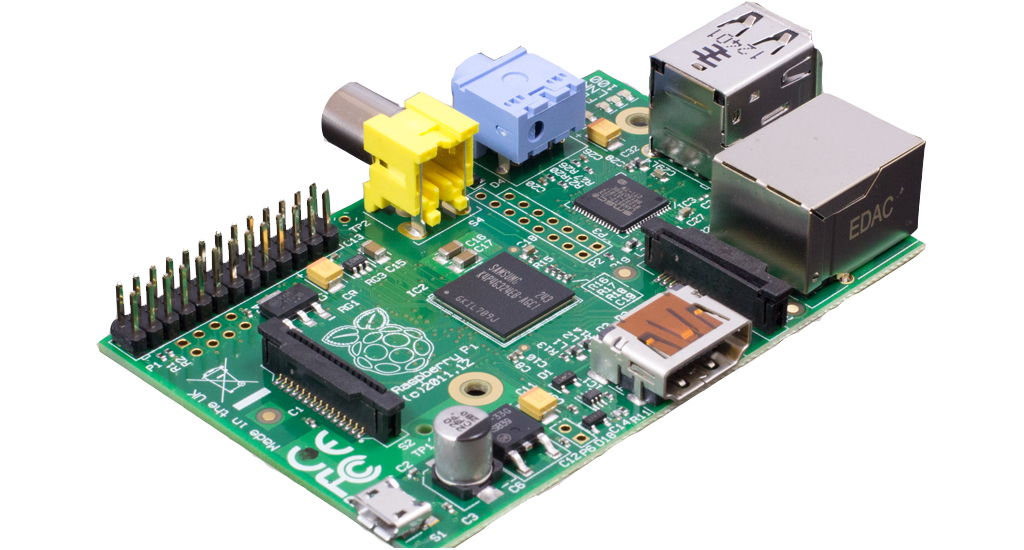
\includegraphics[scale=0.2]{images/raspi.png} 
\caption{Raspberri Pi}
\label{fig:Raspberry Pi}
\end{figure}

\subsubsection{Caracter'isticas}
Aunque existen varios modelos de Raspberry Pi, este proyecto se basa en el modelo B (segunda revisi'on). Este modelo se caracteriza por:

\begin{figure}[ht]
\centering
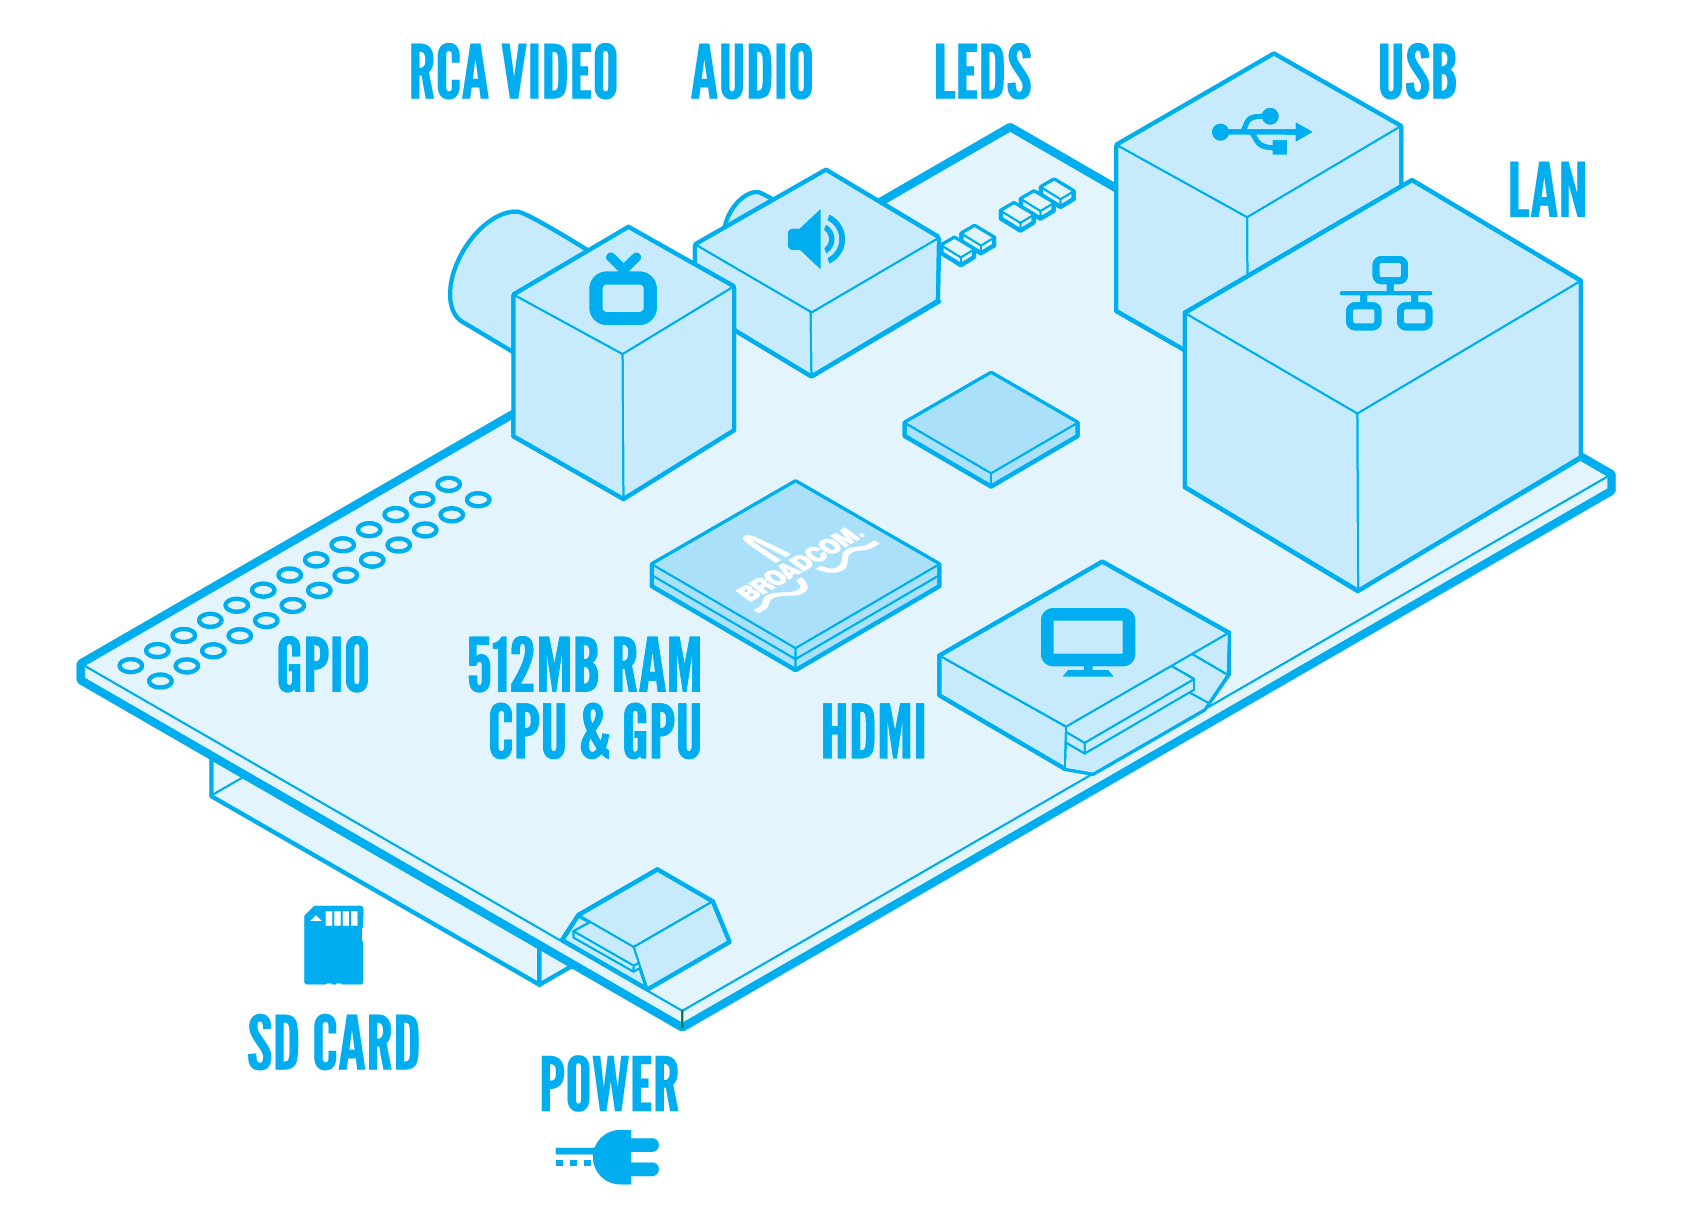
\includegraphics[scale=0.15]{images/RaspiModelB.png} 
\caption{Esquema Modelo B}
\label{fig:Esquema Modelo B}
\end{figure}

%\begin{multicols}{2}
\begin{itemize}
\item Procesador Broadcom BCM2835 (SoC) compuesto por:
	\begin{itemize}
	\item CPU: ARM1176JZF-S (Arquitectura ARM 11)
	\item GPU: VIDEOCORE IV (250 Mhz)
	\item Mem'oria RAM de 512MB
	\end{itemize}
\item Connexiones multimedia:
	\begin{itemize}
	\item 1x Entrada de v'ideo: CSI
	\item 3x Salidas de v'ideo: RCA, HDMI y DSI
	\item 2x Salida de audio: 3.5mm jack y HDMI
	\item 1x RS232
	\end{itemize}
\item Connexiones de datos:
	\begin{itemize}
	\item 1x Ranura tarjeta SD (Disco Duro)
	\item 2x Puertos USB 2.0
	\item 1x Puerto Ethernet RJ45 (10/100 MBit/s)
	\end{itemize}
\item Perif'ericos de bajo nivel:
	\begin{itemize}
	\item 8x GPIO
	\item 1x UART
	\item 1x I$^{2}$C bus
	\item 1x SPI bus (dos pines de selecci'on)
	\end{itemize}
\item Otros datos:
	\begin{itemize}
	\item Alimentaci'on: 5V via MicroUSB o GPIO
	\item Medidas: 85.6mm x 56mm
	\item Peso: 45 g
	\end{itemize}
\end{itemize}
%\end{multicols}



\newpage

\subsection{Protocolos de comunicaci'on}

\newpage

\section{Especificaciones}
Tal y como se ha definido anteriormente, el objetivo de este proyecto consiste en ofrecer una plataforma funcional para los futuros usuarios. Para definir esta ''funcionalidad'' se ha basado en el conocimiento aportado por antiguos usuarios, trabajadores en productos similares y en la experiencia propia. \\

Las especificaciones se han clasificado seg'un su or'igen. Dependiendo de si son de car'acter \textbf{software}, \textbf{electr'onico} o \textbf{mec'anico}. Las especificaciones de car'acter inform'atico engloban aspectos como la interf'icie con el usuario, las herramientas de desarrollo (librer'ias, documentaci'on) y la disponibilidad a futuras modificaciones. Por contra, la electr'onica ha de evitar que el usuario se encuentre obligado a manipular el interior del robot, pero que en el caso de dicha situaci'on permita una soluci'on simple del problema. Adem'as, la electr'onica ha de incorporar un sistema que permita conocer estados del robot de manera sencilla. Finalmente, la mec'anica se encarga de incorporar las nuevas especificaciones en la plataforma, manteniendo el concepto inicial. Igual que en la electr'onica, en el caso de una futura manipulaci'on por parte del usuario, el dise'no ha de facilitar el acceso a cualquier ubicaci'on.

\subsection{Software}
El principal requisito del software es ofrecer un acceso simple al usuario. Teniendo presente el hecho que pueda ser utilizado tanto para usuario noveles como para usuarios experimentados. Por ello se ha planteado las siguientes especificaciones.

\subsubsection{Web}
Se ofrecer'a un servidor web que permita de visualizar f'acilmente el estado del robot como por ejemplo: el nivel de carga de bater'ias, sensores de proximidad, velocidad de desplazamiento, consumo de motores, etc. Adem'as se incluir'a una pantalla d'onde se monitorizar'a una c'amara que incorpora el robot y un par de terminales de comandos.
En otro apartado de la web se ofrecer'a la descarga de todos aquellos documentos necesarios para el usuario, evitando as'i que el usuario pierda tiempo en la b'usqueda de la documentaci'on.

\subsubsection{Librer'ias}
%Por facilidad de uso y comodidad se ha decidido que todo el software utilizado en este proyecto se base en $Python^{ TM}$, un lenguaje de programación
Para aquel desarrollador que decida utilizar esta plataforma se le ofrecer'a un conjunto de librer'ias que permitan trabajar con el robot de manera comoda. Estas librer'ias se compondr'an de una sintaxis limpia y un c'odigo legible que proporcinar'a una f'acil interpretaci'on.    

\subsection{Electr'onica}
El objetivo de la electr'onica es ser la parte m'as vital de la plataforma, pero pasando desapercibida por el usuario. Ofreciendo una m'inima interacci'on pero suficiente para comprender el estado del robot. Esta interacci'on se har'a mediante se'nales luminosas o ac'usticas, e indicar'an los siguientes estados.

\subsubsection{Funcionamiento}
En la plataforma de partida no se dispone de ning'un medio que indique si se encuentra operativo, por ello la primera especificaci'on de la parte electr'onica ser'a la incoporaci'on de un se'nal luminosa que muestre si el robot est'a encendido o apagado. Tambi'en existe la posibilidad de ofrecer informaci'on de otros estados.

\subsubsection{Alimentaci'on}
Las bater'ias ofrecer'an  una autonom'ia suficiente para moverse en un entorno exterior, se estipula un m'inimo de 2 horas en movimiento como m'inimo aceptable. Adem'as de la duraci'on, su recarga deber'a de ser lo m'aximo de comodo para el usuario, evitando que tenga que manipular las celdas de energ'ia. Se recomienda elementos de seguridad ante problemas como sobrecargas o cortocircuitos y de gesti'on de energ'ia para aumentar la vida 'util.\\

Otro punto a tener en cuenta es la disponibilidad en encontrar repuestos de la bater'ia, por ello se usar'an productos comerciales f'aciles de adquirir. Finalmente, se monitorizar'a el nivel de carga a partir de unos elementos luminosos.

\subsubsection{L'ogica}
Para el control de la plataforma el proyecto se ha basa en uso de la Raspberry Pi. Dicho ordenador ser'a el responsable de efectuar todo los c'alculos y 'ordenes, A'un as'i, a causa de sus limitaciones se precisa de una l'ogica complementaria capaz de gestionar y contabilizar las lecturas anal'ogicas de los sensores, el control de motores, la comunicaci'on externa y la distribuci'on de energ'ia.

\subsubsection{Comunicaci'on}  
Para poder interaccionar con el plataforma rob'otica se proponen 3 medios alternativos. Cada uno de estos canales permitir'an el acceso al usuario. Un primer medio ser'a por via cableada, a partir de un cable de red, los otros dos ser'an por via inal'ambrica, por un lado se buscar'a un red Wi-Fi predefinida y por otro se crear'a una red Wi-Fi propia. 

\subsection{Mec'anica}
Se intentar'a en la medida de lo posible mantener la silueta caracter'istica del robot, asignando mayor prioridad a aquellas modificaciones motivadas por software o  electr'onica. 

\subsubsection{Estructura}
Se desea mantener la estructura b'asica de la plataforma, dejando su peculiar forma de dos bloques unidos por una barra roscada longitudinal. Se mantendr'a el concepto de perfiles cuadrados como elemento estructural pero modificando la separaci'on entre ellos.La ubicaci'on de los distintos elementos se dispondr'an seg'un su relaci'on con el resto de dispositivos, uniendo seg'un se traten de control de potencia, l'ogica o comunicaci'on.


\subsubsection{Tornilleria}
A causa del deterioro de los elementos de tornilleria se proceder'a a cambiar el roscado de todos los tornillos por uno m'as estandarizado como el m'etrico. Este cambio tambi'en incluye las barras estructurales, los adaptadores de los ejes y los prisioneros



\newpage
\section{Modificaciones}
Para la realizaci'on de este proyecto se deber'a trabajar en varios sectores. Debido que el software es el sector que permite mejor adaptarse a los nuevos cambios y que la mec'anica de la plataforma proporciona cierta flexibilidad, el componente electr'onico ser'a el que ofrezca las mayores limitaciones. Por ello se considera que los primeros esfuerzos deber'an centrarse en este sector, aprovechando al m'aximo los recursos ya existentes.


Aunque la platafoma inicial segu'ia funcionando, los problemas derivados de su desgaste propiciaron la necesitad de modificar en gran medida su interior. En un principio de demostr'o que simplemente insertando una Raspberry Pi, conectada mediante puerto ethernet, se pod'ia comandar el robot. Tambi'en fu'e posible acceder a datos b'asicos del robot como el estado de las bater'ias o la lectura de los sensores de proximidad. Pero el hecho de la inestabilidad de su unidad de procesamiento hizo necesaria su subtituci'on completa. A causa de a esta decisi'on, se tuvo que buscar el modo de comunicarse con los dem'as componentes ya existentes: etapa de alimentaci'on, gestor de bater'ias, control de motores y lectura de sensores. 

\subsection{ Componentes Electr'onicos}
Para poder actuar con cada dispositivo, el robot hac'ia uso de las interf'icies de comunicaci'on UART e I$^{2}$C; Pero a'un sabiendo el protocolo empleado, la comprensi'on de la informaci'on que circulaba fu'e pr'acticamente imposible. Por ello se determin'o que para poder proseguir con el proyecto hac'ia falta el desarrollo de nuevos componentes que substituyesen a los actuales y que permitiesen a futuros usuarios comprender r'apidamente que protocolos se utilizan y c'omo interaccionar con ellos. A continuaci'on se detallan los componentes utilizados.

\subsubsection{Motorizaci'on}
Debido al buen estado de los motores y del hecho que un par incorpora codificadores de cuadratura, se ha optado por mantener estos motores. Con este gesto evitamos la b'usqueda de su substituto y nos aseguramos que se mantenga la misma funcionalidad que al inicio. Al conservar este dispositivos se considera que el consumo (por lo que afecta a la parte de motorizaci'on) permanecer'a semejante, por tanto la nueva etapa de control de motores dispondr'a de características similares. Siendo el voltaje nominal del grupo motriz de unos 7.2 se requiere de una alimentaci'on acorde a este voltaje; En el caso de utilizar bater'ias de voltaje superior, ser'a necesario una etapa DC-DC para adecuar los niveles.


\subsubsection{Sensores de proximidad}
Cualquier plataforma rob'otica dedicada a la exploraci'on ha de disponer de sensores que les proporcionen informaci'on sobre el mundo que le rodea. Por ello se aprovechar'an los sensores anal'ogicos infrarrojos actuales del robot, Sharp GP2Y0A2YK, y se an'adir'an cuatro nuevos sensores por ultrasonidos KS103.\\

\begin{figure}[ht]
\centering
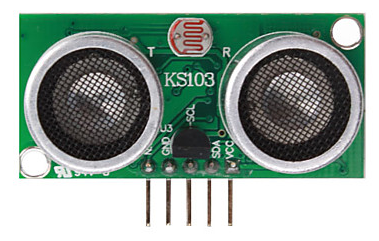
\includegraphics[scale=0.40]{images/KS103.png}
\caption{Sensor de distancia por ultrasonidos KS103}
\label{fig:KS103}
\end{figure} 

Las caracter'isticas de este sensor han sido el motivo de su elecci'on: Su gran rango de medida (de 1cm a 550cm), una resoluci'on de 1mm, comunicaci'on via I${^2}$C (con 20 direcciones possibles), capaz de operar de 3.0 a 5.5V y permite hasta unas 500 lecturas por segundo. Otro factor que se ha tenido en cuenta es el hecho que la luz de sol en determinadas circunstancias puede afectar a la lectura real de los sensores infrarrojos, en cambio los sensores de ultrasonidos no quedan afectados.\\

\begin{figure}[ht]
\centering
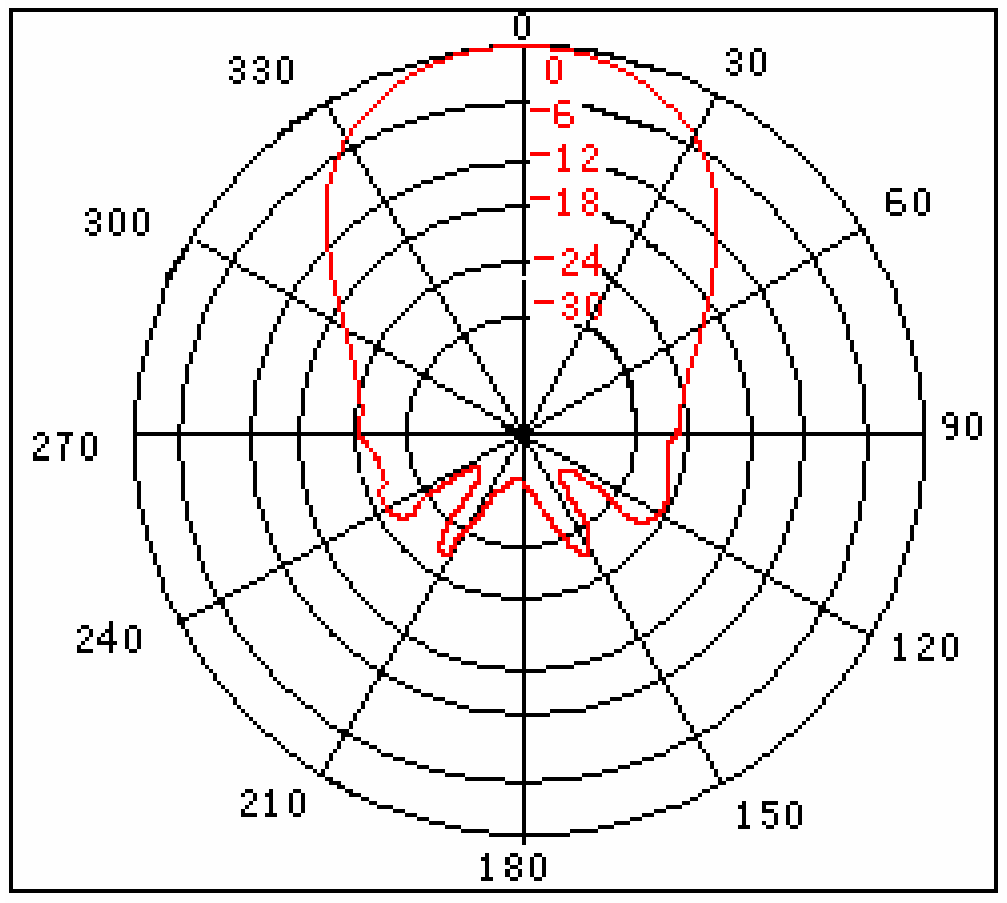
\includegraphics[scale=0.20]{images/KS103_diagram.png}
\caption{Diagrama de radiaci'on del sensor KS103}
\label{fig:KS103_diagram}
\end{figure} 

El funcionamiento de este tipo de sensor de basa en el envi'o de un pulso y la recepci'on de su eco, luego el propio sensor determina el tiempo entre estos dos sucesos y calcula la distancia a la que se encuentra el obst'aculo. Debido a que los ultrasonidos producidos pueden afectarse entre ellos si se realiza una lectura simult'anea, se deber'a esperar la finalizaci'on de la lectura de un sensor para activar el siguiente. 



\subsubsection{Bater'ia}
Para la selecci'on del sistema de acumulaci'on de energ'ia se ha barajado diferentes posibilidades que podemos encontrar en el mercado:Bater'ias de plomo, NiCd, NiMH, Ion Litio y Pol'imero de Litio (LiPo). Las de plomo han sido las primeras descartadas a causa de su baja densidad de carga y su elevado peso. Las constituidas por elementos de NiCd se encuentran en fase de desaparici'on por experimentar el efecto mem'oria (reducci'on de su capacidad al cabo del tiempo) y ser superadas por sus competidoras. Las bater'ias de Ion de Litio, a'un disponiendo de una alta densidad de carga y bajo peso (motivo de su extendido uso en dispositivos m'obiles), no son capaces de ofrecer una gran capacidad de descarga. \\

\begin{table}[ht]
\begin{center}
\begin{tabular}{|c|c|c|}
	\hline
	\textbf{Tipo} & \textbf{Densidad de carga} & \textbf{Densidad de potencia} \\ 
	\textbf{ } & \textbf{[Wh/Kg]} & \textbf{[W/Kg]} \\	\hline
	NiCd & 50 & 600 \\ \hline
	NiMh & 70 & 700 \\ \hline
	Li-Ion & 220 & 300 \\ \hline
	Li-Poly & 150 & 2690 \\ \hline

\end{tabular}
\end{center}

\caption{Comparativa entre tipos de bater'ias }
\label{tab:Battery_type_table}
\end{table}

Llegados a este punto queda decidir entre las bater'ias constituidas por NiMH o LiPo. Ambas bater'ias est'an ampliamente comercializadas y ofrecen una alta capacidad de descarga si se comparan con las descartadas. Aunque las LiPo disponen de mejores caracter'isticas, seg'un la tabla \ref{tab:Battery_type_table}, se corre el riesgo de que  lleguen a incendiarse si se sobrecargan o que queden inutilizadas si se alcanza un voltaje inferior de 2.5V por celda.\\

\begin{figure}[ht]
\centering
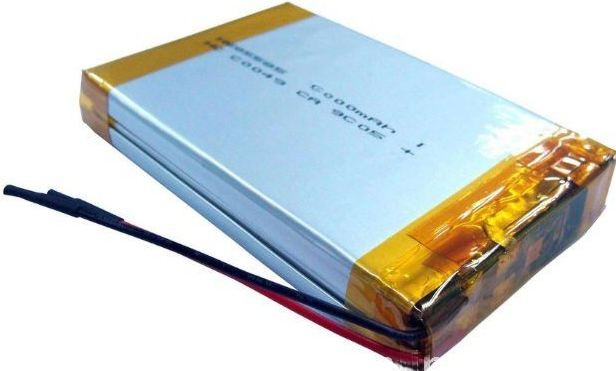
\includegraphics[scale=0.4]{images/Lipo_PCM.png} 
\caption{Bater'ia LiPo con PCM instalado}
\label{fig:LiPo_PCM}
\end{figure} 

Por ello se ha optado por el uso de unas bater'ias con un m'odulo PCM instalado, este peque'no dispositivo ofrece un control sobre la bater'ia, protegi'endola de sobredescargas y gestionando su carga. Adem'as ya no hace necesario cargadores espec'ificos, simplemente una fuente de tensi'on acorde. Debido a que los motores tienen un voltaje nominal de 7.2V, se ha decidido el uso de bater'ias de 7.4V, estas bater'ias tienen un rango de funcionamiento de 2.75 hasta los 4.2V. \\

Finalmente las la bater'ia elegidas ha sido un conjunto formado por dos celdas de 3.7V de 6000mAh cada una conectadas en serie y con un modulo PCM instalado. Su consumo de carga llega a los 2A y a unos 6A en descarga.

\subsubsection{Punto de acceso WiFi}
Tal y c'omo se ha descrito en las especificaciones, se requiere de una sistema que ofrezca un acceso WiFi. Debido a que se ha descartado el uso del m'odulo que ya dispo'ia el robot, se hace necesario un nuevo dispositivo que se encargue. En este caso de ha optado por el uso de un elemento comercial de tama'no reducido que se pueda alimentar f'acilmente, ofezca un alcance aceptable y de r'apida configuraci'on.

\begin{figure}[ht]
\centering
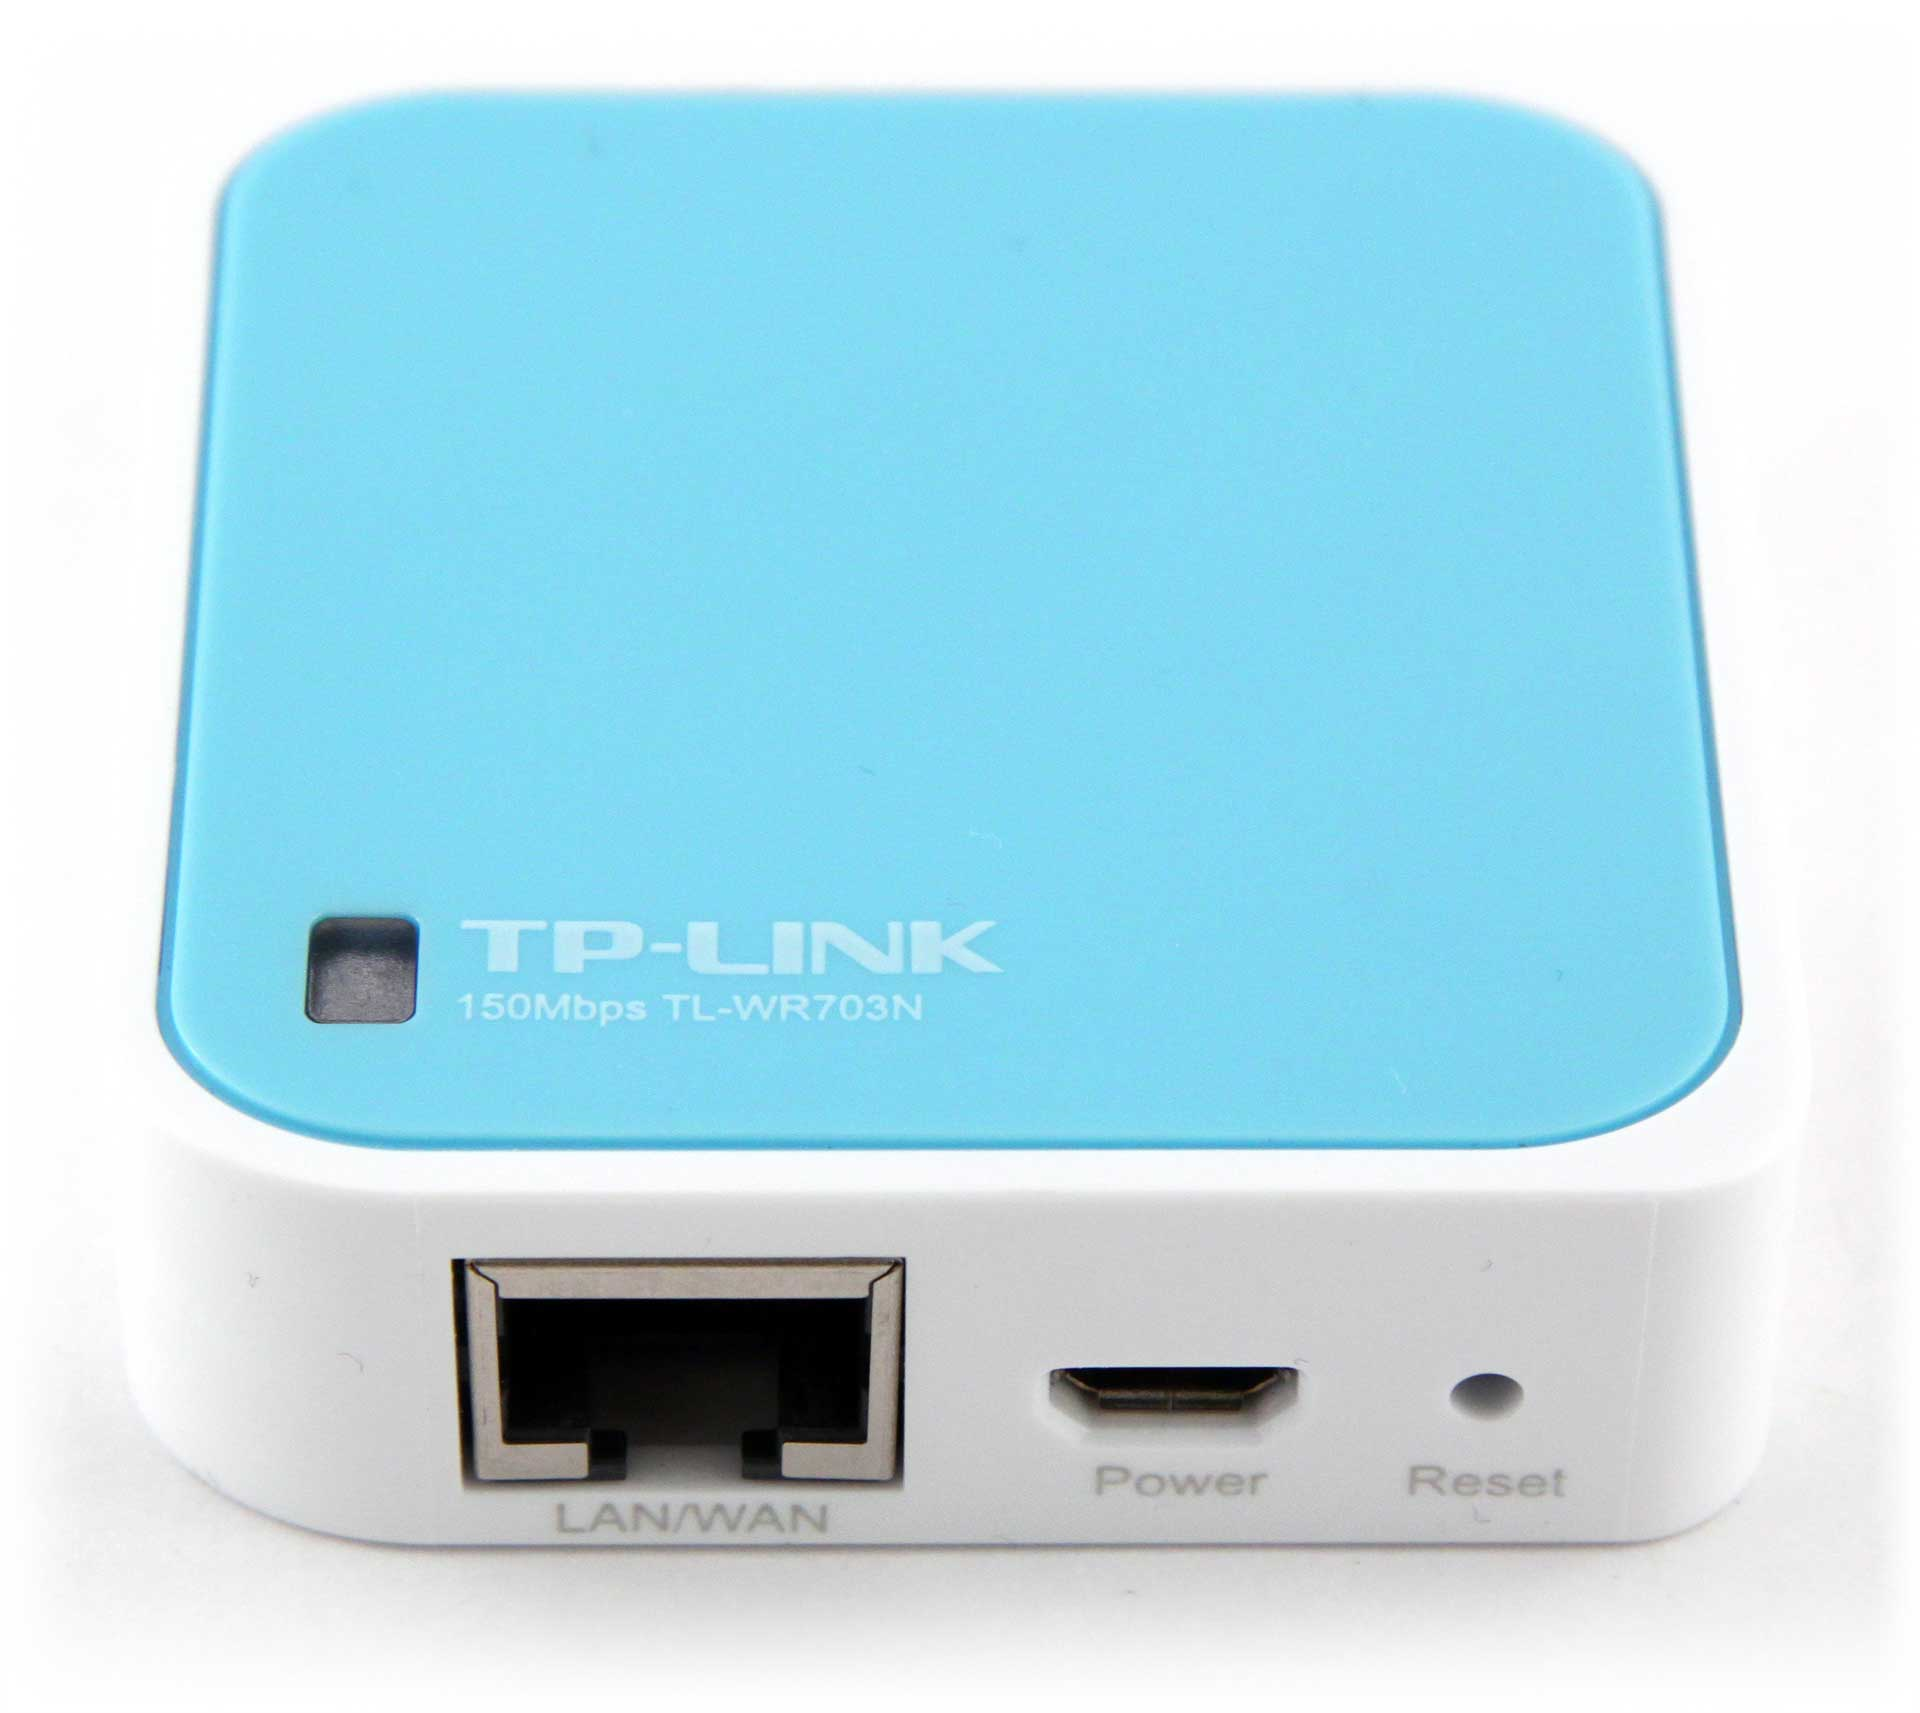
\includegraphics[scale=0.15]{images/TL-WR702N.png} 
\caption{Router TP-Link WR702N}
\label{fig:TL-WR702N}
\end{figure}

El dispositivo elegido se trata del mini router TL-WR702N de la empresa TP-LINK. Este modelo ofrece una velocidad m'axima de transmisi'on de 150Mbps, se alimenta mediante un puerto MicroUSB (5V) y dispone de un puerto ethernet RJ45, que dependiendo del modo de trabajo se comporta como un puerto WAN o LAN.\\

Entre todas sus configuraciones (AP Mode, Router Mode ,Client Mode,
Repeater Modey  Bridge Mode) se ha optado por la de punto de acceso con el nombre de RosPiBot y servidor DHCP activado. De esta manera el usuario s'olo deber'a conectarse a su red para poder acceder al robot.

\subsubsection{Conmutador de red}
Seg'un las especificaciones se desea que la nueva plataforma disponga de tres medios de acceso a red. Dos de estos medios (Wifi y clavija ethernet) han de estar conectados directamente con el puerto ethernet de la Raspberry, por este motivo se necesita un conmutador o switch. Puesto que el robot ya dispone de un switch de 5 puertos (4 habilitados), se aprovechar'a el mismo dispositivo.\\

\begin{figure}[ht]
\centering
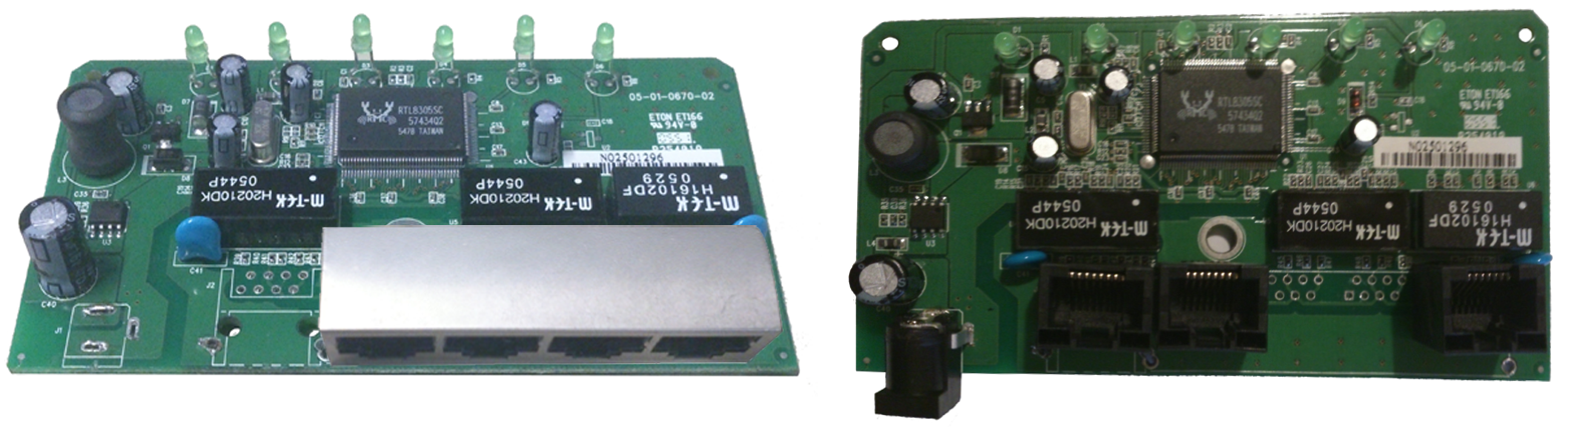
\includegraphics[scale=0.35]{images/switch_comparative.png} 
\caption{Switch antes y despu'es de la modificaci'on}
\label{fig:switch_comparative}
\end{figure}

Debido a que el conector que dispone el switch implica una que el conector se encuentre en posici'on horizontal, se ha optado por la substituci'on de la clavija de cuatro puertos por tres verticales, de esta manera se reduce la superf'icie que requiere el switch con los conectores.

\subsubsection{Descodificador de cuadratura} \label{sec:LS7366}
Uno de los elementos m'as 'utiles que podemos encontrar en la plataforma es la existencia de dos codificadores de cuadratura dispuestos en el grupo motriz delantero (uno a cada lado). Estos dispositivos permiten medir los cambios del eje del motor (antes de la etapa reductora) con gran precisi'on. Para su funcionamiento requieren de una alimentaci'on de 5 voltios, siendo este mismo voltaje el usado en la salida del se'nal. Debido a su voltaje, superior a los 3.3 voltios que soportan los pines de la Raspberry Pi, se hace necesario un adaptador de nivel. Adem'as, seg'un los resultados experimentados, la frecuencia m'axima de interrupciones generadas por el codificador llega hasta las 80.000 por segundo, Haciendo imposible que el microprocesador sea capaz de gestionarlo.

\begin{figure}[ht]
\centering
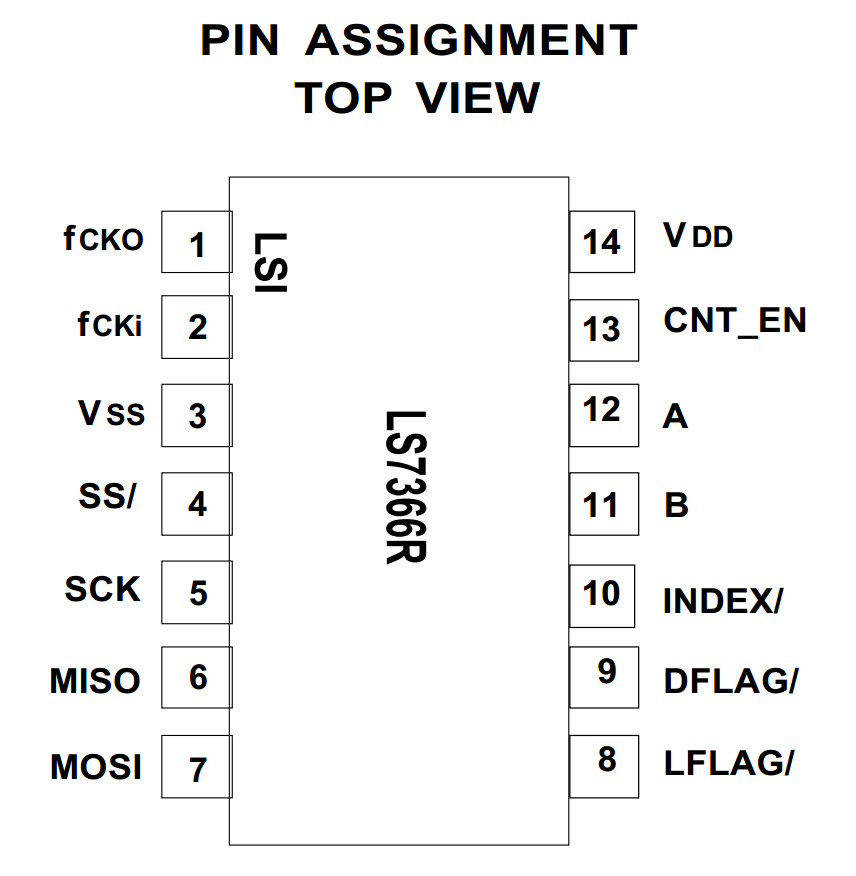
\includegraphics[scale=0.15]{images/LS7366.png} 
\caption{Diagrama de pines LS7366}
\label{fig:LS7366}
\end{figure} 

Para solventar el problema, se hace uso del circuito integrado LS7366, un contador de cuadratura de hasta 32 bits con interf'icie SPI. Este componente incrementa o decrementa un contador interno dependiendo de la secuencia que proviene del codificador de cuadratura. Adem'as en el momento que se quiera acceder al registro de dicho contador, el circuito procede a copiar el estado de contador en un segundo registro, permitiendo que la lectura no interfiera con el c'omputo.\\

Gracias a este integrado, se evita que el microprocesador tenga que hacerse cargo del gran nombre de interupciones, permiti'endole dedicarse a otros procesos. Para la comunicaci'on se aprovecha el m'odulo propio SPI del BCM2835 y dos de los pines de selecci'on de escalvo. 

\subsubsection{Adaptador de nivel de tensi'on}
Para una correcta comunicaci'on entre los diferentes dispositivos es preciso adaptar los diferentes voltajes. Para ello hay que tener en cuenta en que rangos cada dispositivo se comunica; Mientras que la Raspberry Pi usa voltajes en su GPIO de 0 a 3.3V, el controlador de motores opera con tensiones superior a los 4.5V.\\

Debido a que algunos pines requieren bidirecionalidad (por ejemplo I${^2}$C) se ha decantado por el uso del circuito recomendado por la empresa \textbf{Philips Semiconductors} explicado en su documento \textbf{AN97055} y que corresponde a la figura \ref{fig:Level_shifter_circuit}. Finalmente para el circuito se utilizar'an resistencias de 10K$\Omega$ para la funci'on de ''pull-up'' y el mosfet de canal N \textbf{BSS138} como el de la figura \ref{fig:BSS138}.

\begin{figure}[ht]
\centering
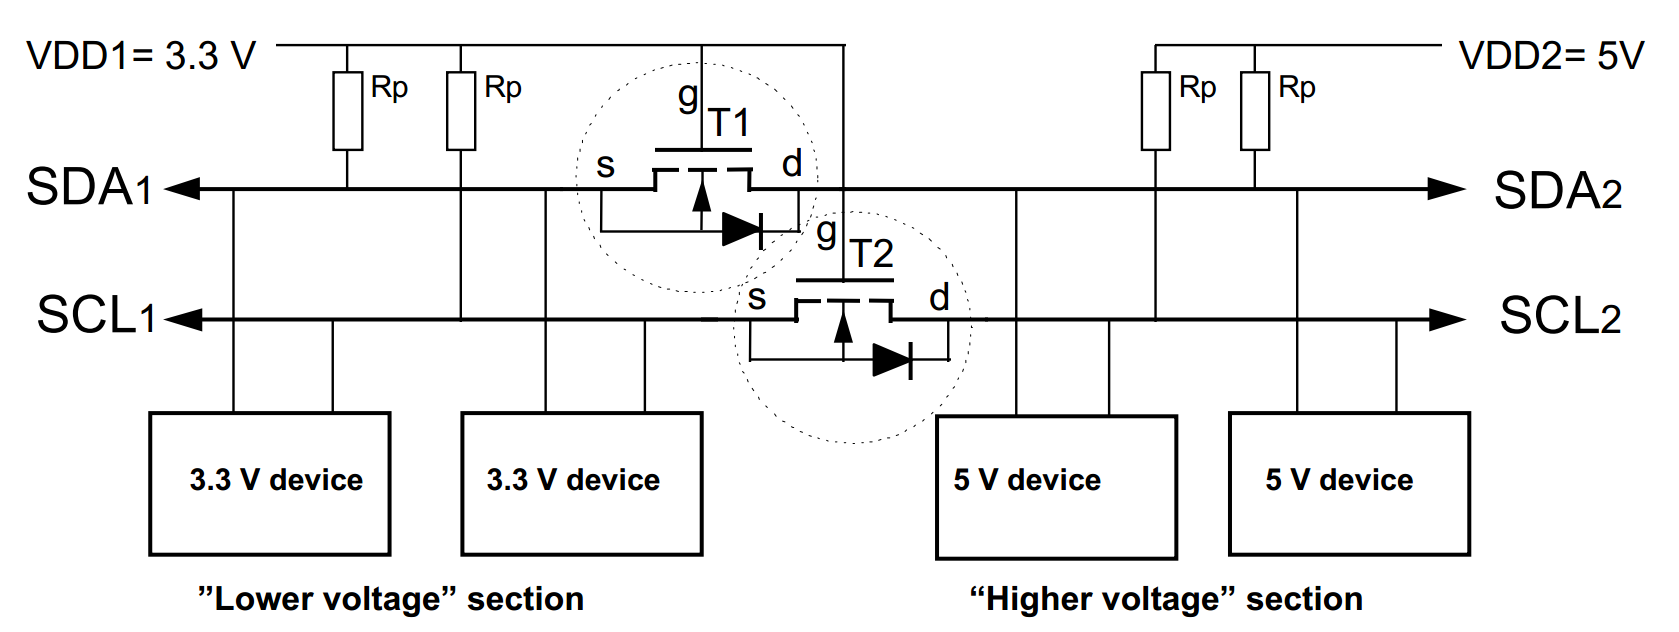
\includegraphics[scale=0.30]{images/level_shifter_circuit.png}
\caption{Circuito adaptador de tensi'on}
\label{fig:Level_shifter_circuit}
\end{figure} 

\begin{figure}[ht]
\centering
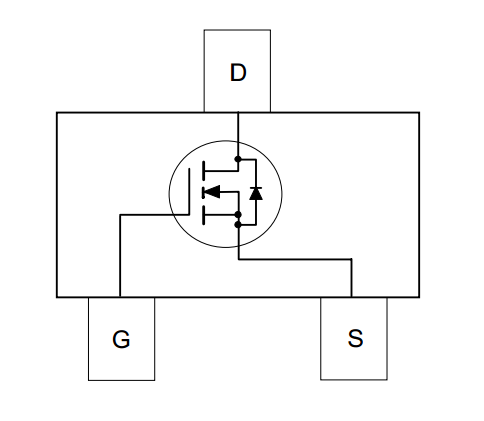
\includegraphics[scale=0.30]{images/bss138_diagram.png}
\caption{Diagrama BSS138}
\label{fig:BSS138}
\end{figure} 

\subsubsection{Lectura de valores anal'ogicos}
Debido al uso de sensores de salida anal'ogica (sensores de distancia por infrarrojos), el uso de resistencias Shunt y la monitorizaci'on de bater'ias, se requiere una lectura anal'ogica. Por ello se utilizar'a un conversor anal'ogico a digital o ADC ya que la Raspberry no dispone de uno propio. De los posibles componentes que cumplan esta funci'on se ha elegido aquel que de comunique por I$^{2}$C, ofrezca una resoluci'on aceptable, haya sido utilizado satisfactoriamente por otros usuarios y de menor coste. El componente elegido ha sido el MCP3428, un conversor ADC Sigma-Delta de 4 canales diferenciales, resoluci'on de hasta 16 bits y voltaje de referencia interno de 2.048 voltios.

\begin{figure}[ht]
\centering
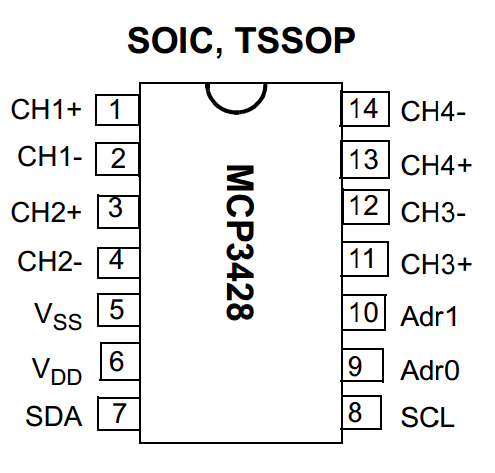
\includegraphics[scale=0.30]{images/MCP3428_pin_diagram.png}
\caption{Diagrama de pines MCP3428}
\label{fig:MCP3428}
\end{figure} 


\subsubsection{Monitorizaci'on de la Bater'ia}
Conocer el estado de la bater'ia en cualquier momento es crucial en plataformas m'oviles, por ello su monitorizaje es imprescindible. Dicho monitorizaje se efectua de dos maneras distintas: La primera mediante un m'odulo ADC que digitaliza el estado de la bater'ia, y la segunda utiliza el circuito integrado LM3914, un dispositivo encargado de medir el voltaje y mostrar dicha informaci'on mediante LEDs.

\begin{figure}[ht]
\centering
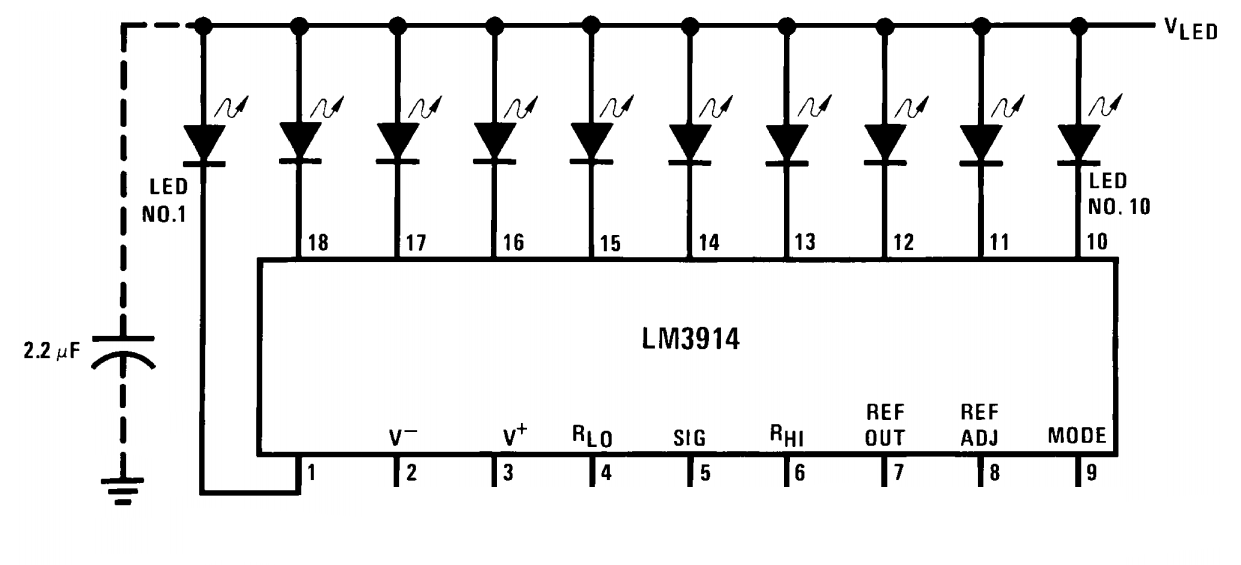
\includegraphics[scale=0.30]{images/LM3914_pin_diagram.png}
\caption{Diagrama de pines LM3914}
\label{fig:LM3914}
\end{figure} 

\subsubsection{Alimentaci'on de l'ogica}
A causa de los diferentes niveles de tensi'on entre la bater'ia que cada componente requiere, se hace necesario un sistema que lo adecue; Por ello se ha dedicido usar un regulador que ofrezca una salida estable de 5 voltios. En el caso de la Raspberry Pi se utilizar'a el propio regulador interno de 5 a 3.3V.
A partir de experimentaciones previas se estima un consumo medio de 1500mA. Para satisfacer dicho consumo es necesario un regulador de alta eficiencia, y debido a que siempre nos encontramos la situaci'on de reducir el voltaje, deberemos usar un convertidor Buck. 

\begin{figure}[ht]
\centering
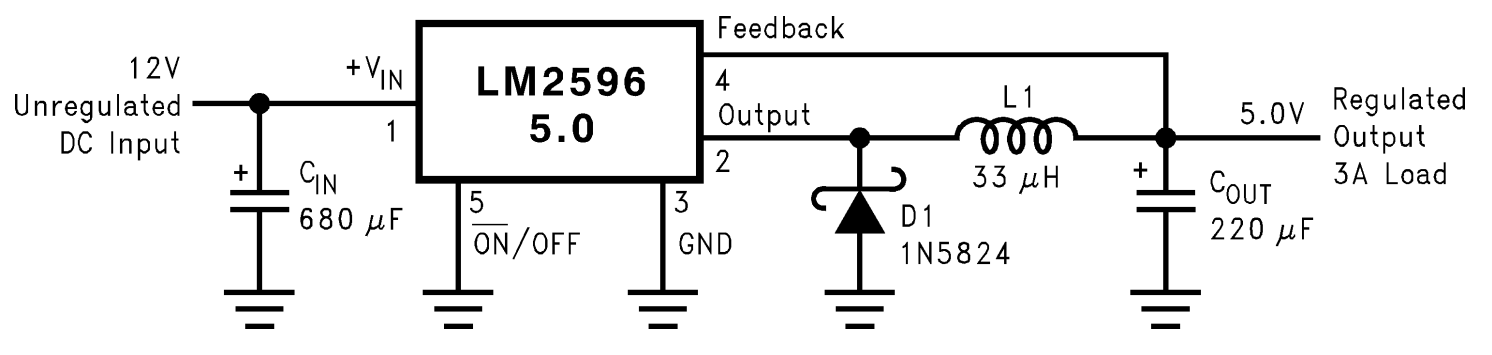
\includegraphics[scale=0.35]{images/LM2596.png}
\caption{Circuito regulador Buck 5V}
\label{fig:LM2596}
\end{figure} 

El componente elegido ha sido el LM2596, un regulador capaz de ofrecer hasta 3A. Su elecci'on se ha basado en el tipo de componentes que requiere, su facilidad de uso, su coste total reducido y la experiencia previa con este regulador. Para la selecci'on de componentes, la mayor'ia vienen definidos por el propio fabricante, excepto la bobina, la  cual para obtener el m'aximo rendimiento del regulador su inductancia se ha de elegir seg'un la figura \ref{fig:Bobina_Graph}. Puesto que las bater'ias oscilan de 6 a 8.4V y que el consumo var'ia de 1 a 2A, se ha coloreado de verde claro aquellas zonas en la que el regulador puede llegar a trabajar y de color m'as oscuro la zona m'as t'ipica d'onde se puede encontrar. Por esto motivo se ha elegido el valor de 22 $\mu$H.

\begin{figure}[ht]
\centering
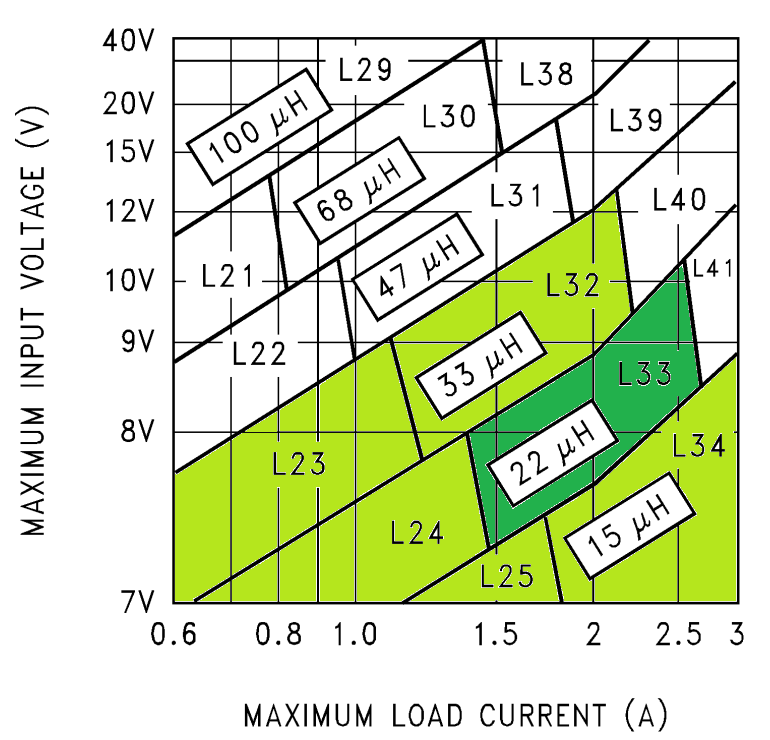
\includegraphics[scale=0.30]{images/bobina_graph.png}
\caption{Guia de selecci'on de inductancia}
\label{fig:Bobina_Graph}
\end{figure} 

\subsubsection{Control de motores} \label{sec:L298N}
Para el control de motores se utilizar'a el mismo componente L298 usado en el robot original, un doble puente en H . Este dispositivo permite un control independiente de dos motores de cont'inua hasta un consumo de 2 amperios por motor.\\

\begin{figure}[ht]
\centering
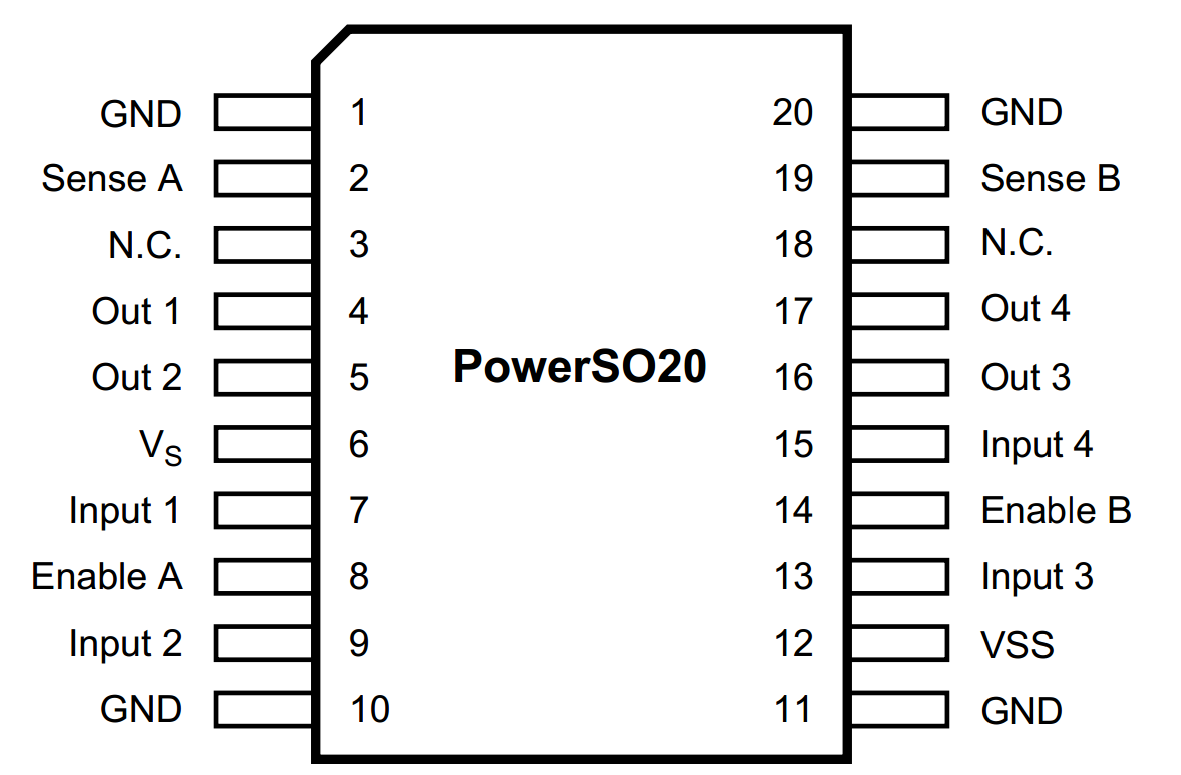
\includegraphics[scale=0.25]{images/L298_pin_diagram.png}
\caption{Diagrama de pines L298N}
\label{fig:L298N}
\end{figure} 

El sentido de rotaci'on se dirige a partir de dos pines indicados como ''Inputs'' y la velocidad mediante una se'nal PWM en el pin de ''Enable''. Aunque dispone de una salida para conocer la intensidad que circula por cada canal (se conecta en serie una resistencia Shunt y se mide la diferencia de potencial), no dispone de ning'un sensor para saber la velocidad del motor.

\subsection{Integraci'on de los componentes}
Los componentes descritos anteriormente desde los puntos \ref{sec:LS7366} hasta \ref{sec:L298N} requieren de ser montados en una PCB. Para ello se han dise'nado un conjunto de placas, se han enviado a producir y finalmente se han ensamblado los componentes manualmente.\\

Para la producci'on de las PCB se ha utilizado un servido de prototipado de bajo coste pero con la limitaci'on que los dise'nos han de estar contenidos en rect'angulos de 5x5, 5x10 o 10x10cm. Aunque posiblemente se pudiera incluir todos los componentes en un solo circuito impreso de 10x5cm, se ha preferido crear 3 dise'nos de 5x5cm. As'i se reduce el riesgo de deshacerse de toda una placa por culpa de un imperfecci'on en un componente y se da modularidad al sistema. Las placas creadas s'on: SecurePi, SensorPi y MotorPi.

\subsubsection{SecurePi}
Esta placa tiene dos objetivos: Ofrecer una etapa de regulaci'on para la alimentaci'on de todos aquellos elementos que requieran una alimentaci'on de 5V y proteger todos los pines GPIO de la Raspberry Pi (ofreciendo bidirecionalidad y convirtiendo el voltaje de 3.3 a 5V).

\begin{figure}[ht]
\centering
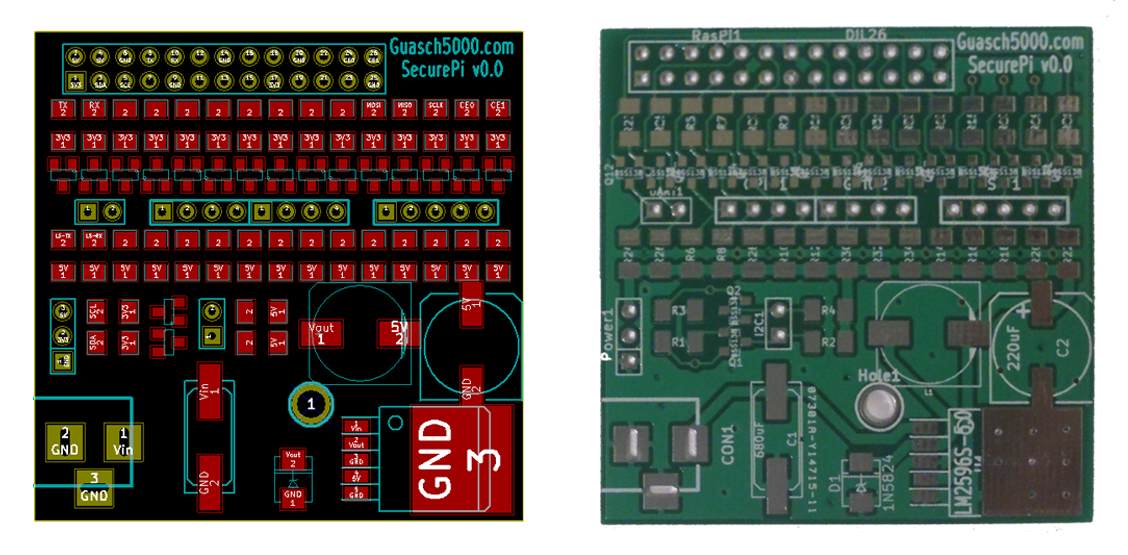
\includegraphics[scale=0.60]{images/SecurePi_comparation.png}
\caption{Layout y PCB de la placa SecurePi}
\label{fig:SecurePi_comparation}
\end{figure} 

Otra caracter'istica de esta placa es la redistribuci'on de los pines, separados seg'un la funcionalidad de cada uno. Podemos observar como el conector de 26 pines se ha distribuido en varios: UART(x2), GPIO(x8), SPI(x5), I2C(x2) y alimentaci'on (GND, 3.3V y 5V).\\

Tal y como se aprecia en la figura \ref{fig:SecurePi_mounted}, una vez montada la SecurePi encima de la Raspberry, el usuario puede seguir accediendo a los pines directos del GPIO, usar las nuevas salidas elevadas a 5V y decidir si alimentar el dispositivo mediante el puerto MicroUSB o con una fuente de mayor tensi'on mediante el conector Jack de 5.1mm.

\begin{figure}[ht]
\centering
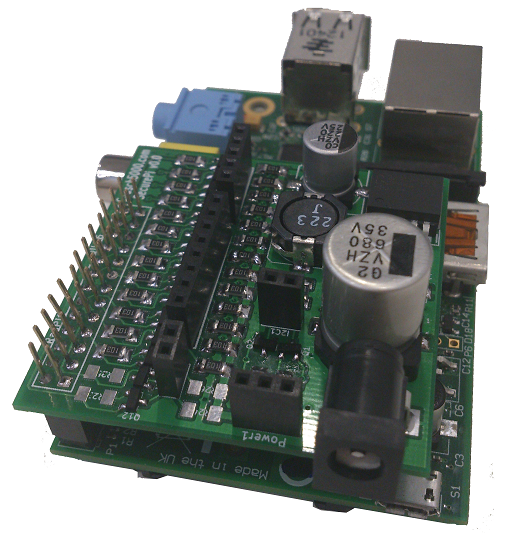
\includegraphics[scale=0.40]{images/SecurePi_mounted.png}
\caption{SecurePi colocada con la Raspberry Pi}
\label{fig:SecurePi_mounted}
\end{figure} 

\subsubsection{SensorPi}
Sobre la placa SecurePi se coloca la SensorPi, esta placa dispone de los descodificadores de cuadratura, los conversores anal'ogicos y un conjunto de leds (uno verde para indicar la correcta alimentaci'on y ocho 'ambar para los pines GPIO destinador a al control de motores).\\

Para cada uno de los descodificadores se han dispuesto de dos tiras de tres pines que disponen de alimentaci'on (GND y 5V), dos canales de cuadratura y un pin opcional para el 'indice. En el caso de las entradas anal'ogicas, se han adaptado mediante divisores de tensiones para ajustar al l'imite de 2.048V. Para medir las bater'ias se han dispuesto de dos lectura para cada una de las celdas en serie, la primera lectura tiene el fondo de escala a 5V y la segunda a 10V. Para los sensores infrarrojos se han configurado a 3.5V como máximo y a 2.2V las dise'nadas para la lectura de la intensidad (midiendo la ca'ida de potencial entre los extremos de una resistencia Shunt). \\

Finalmente las ocho salidas del GPIO se han colocado en un extremo para facilitar su acceso y se ha dispuesto una tira de 4 pines extra para la alimentaci'on y comunicaci'on de los dispositivos que utilizan I${^2}$C.   


\subsubsection{MotorPi}

\subsection{Conexionado}

\newpage


\section{Presupuesto}
\newpage

\section{Conclusiones}
\newpage

\section{Agradecimientos}
\newpage

\section{Biografia}
\newpage

\section{Soporte inform'atico}

\end{document}
